\section{Distance to nearest atom}
\todoa{Mention that images are made with no water molecules (only passivation atoms) in system}

We have made 3d maps of the system labelled ``rough fracture \#2'', using the method from \cref{sec:distance_to_atom}, which finds the distance to the nearest atom on a grid of points. The results can be seen in \cref{fig:distance_to_atom_r05,fig:distance_to_atom_r20}, where we show slices of the maps in the $yz$- and $xy$-plane. For the first figure we used a max distance of 5 \AA, while for the second one we used a max distance of 20 \AA. The maps were made from the molecular system after cutting out the atoms to make the pore and passivating the dangling ends, but before filling the pore with water. A similar map can me made by not including the water molecules in the calculations.

In \cref{fig:distance_to_atom_r05} we can clearly see the positions of the atoms in the silica matrix as the dark blue dots, while the pores light up as red areas.

In \cref{fig:distance_to_atom_r20} we still see the positions of the atoms, but they are less visible now since we have a bigger range for the colormap. We can still see the pores easily, colored white, and we now also see some characteristics of the pore itself, where it has a darker red color.
%
%
% \setlength{\myfigwidth}{1.0\textwidth}%
% \begin{figure}[htpb]%
%     \centering%
%     \includesvg[pretex=\normalsize, width=\myfigwidth, svgpath = ./images/distance_to_atom/rough_fracture_03/]{05_r05_n256}%
%     \caption{%
%         A slice of  $r = 5$ \Ang%
%     }%
%     \label{fig:distance_to_atom_r05}%
% \end{figure}%
% %
% \begin{figure}[htpb]%
%     \centering%
%     \includesvg[pretex=\normalsize, width=\myfigwidth, svgpath = ./images/distance_to_atom/rough_fracture_03/]{05_r20_n256}%
%     \caption{$r = 20$ \Ang}%
%     \label{fig:distance_to_atom_r20}%
% \end{figure}%
%
\begin{figure}[htpb]%
    \centering%
    \setlength{\myfigwidth}{0.9\textwidth}%
    \begin{subfigure}[b]{\myfigwidth}%
        \includesvg[pretex=\normalsize, width=\textwidth, svgpath = ./images/distance_to_atom/rough_fracture_03/]{05_r05_n256}%
        \caption{Max distance $r_\text{max}=5.0$ \AA.%
        \label{fig:distance_to_atom_r05}}%
    \end{subfigure}%
    \vspace{10pt}
    \begin{subfigure}[b]{\myfigwidth}%
        \includesvg[pretex=\normalsize, width=\textwidth, svgpath = ./images/distance_to_atom/rough_fracture_03/]{05_r20_n256}%
        \caption{Max distance $r_\text{max}=20$ \AA.%
        \label{fig:distance_to_atom_r20}}%
    \end{subfigure}%
    \caption{%
        Slices of 3d maps of the distance to the nearest atom in the system labelled ``rough fracture \#2'', generated using method program from \cref{sec:distance_to_atom}, using a colormap that goes from \textbf{a)} 0 to 5 \AA, and \textbf{b)} 0 to 20 \AA. \hl{FINISH CAPTION}%
    }%
\end{figure}%


% %
% \begin{figure}[htpb]%
%     \centering%
%     \setlength{\myfigwidth}{0.49\textwidth}%
% %     \setlength{\mycaptionwidth}{0.3\textwidth}%
% %
%     \begin{subfigure}[b]{\myfigwidth}%
%         \centering% % Need to center to get image centered over caption
%         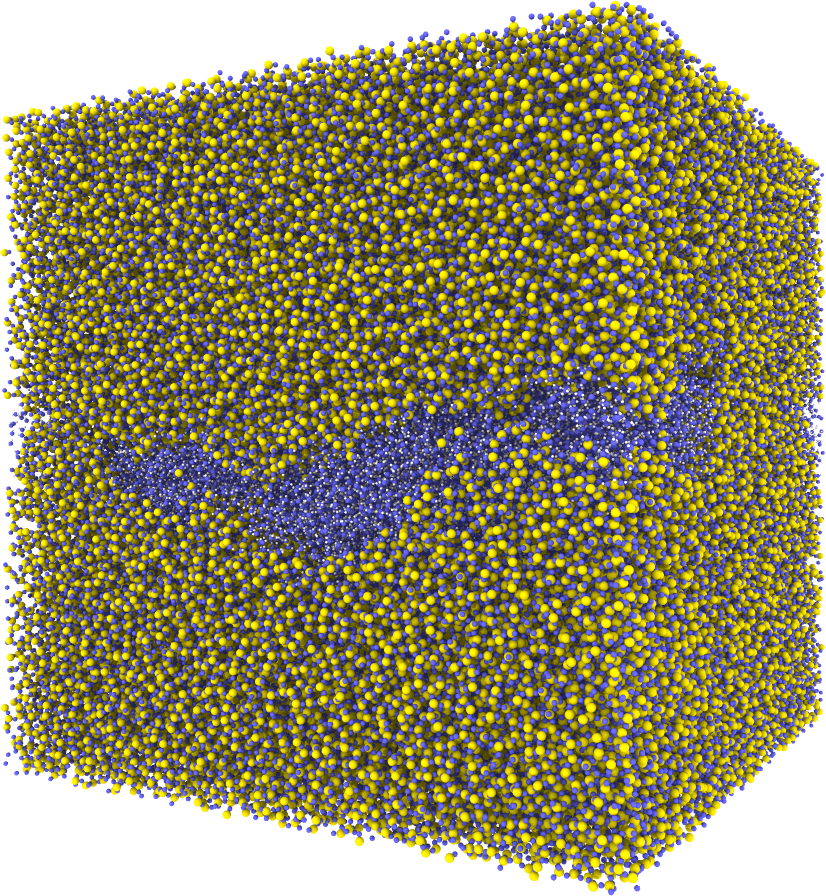
\includegraphics[width=\textwidth]{images/systems/trimmed-rough_fracture01_abel_13}%
%         \caption{Caption.}%
% %         \label{fig:hex_to_tetra}%
%     \end{subfigure}%
%     \hfill%
%         \begin{subfigure}[b]{\myfigwidth}%
%         \centering% % Need to center to get image centered over caption
%         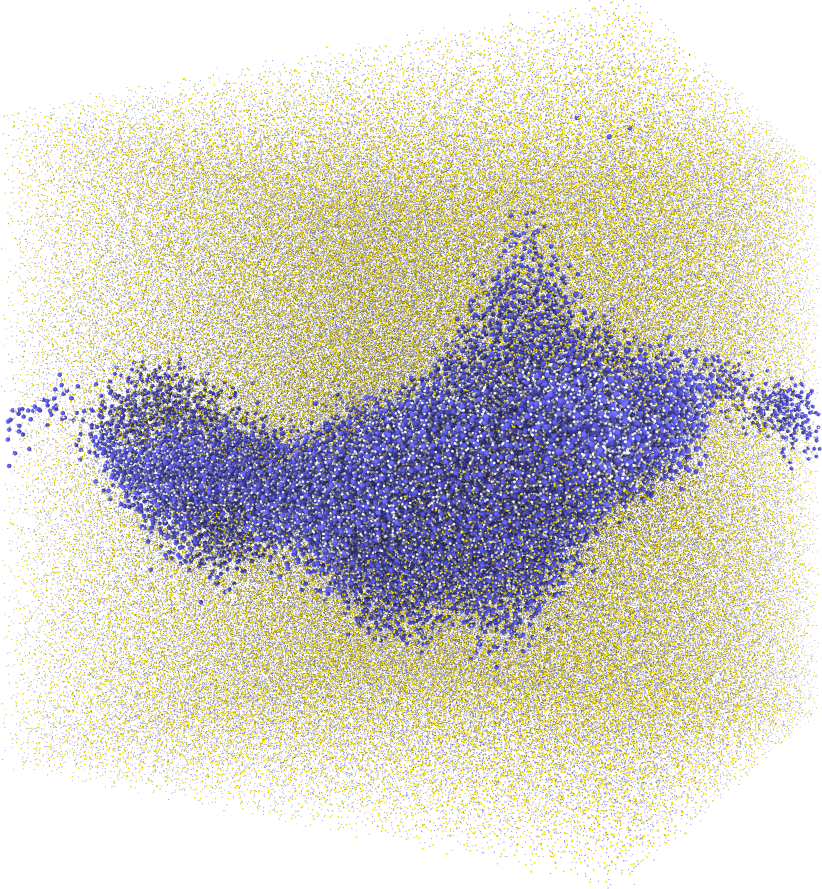
\includegraphics[width=\textwidth]{images/systems/trimmed-rough_fracture01_abel_15}%
%         \caption{Caption.}%
% %         \label{fig:hex_to_tetra}%
%     \end{subfigure}%
%     \\%
%     \begin{subfigure}[b]{\myfigwidth}%
%         \centering% % Need to center to get image centered over caption
%         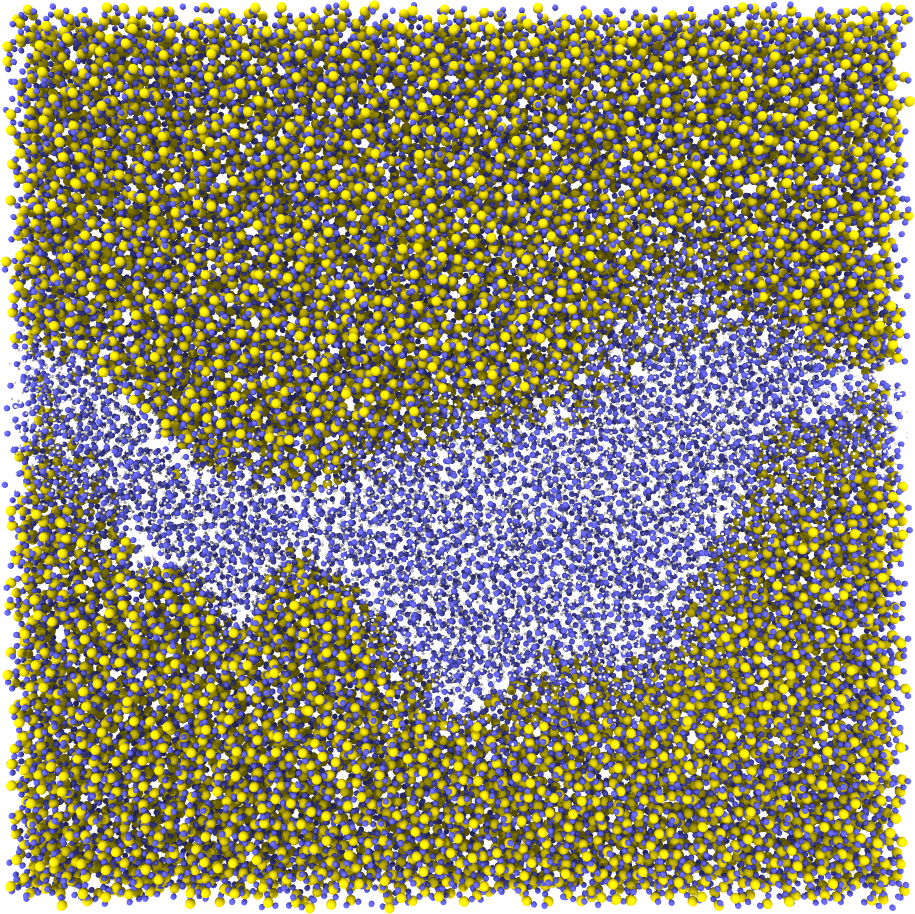
\includegraphics[width=\textwidth]{images/systems/trimmed-rough_fracture01_abel_16}%
%         \caption{Caption.}%
% %         \label{fig:hex_to_tetra}%
%     \end{subfigure}%
%     \hfill%
%     \begin{subfigure}[b]{\myfigwidth}%
%         \centering% % Need to center to get image centered over caption
%         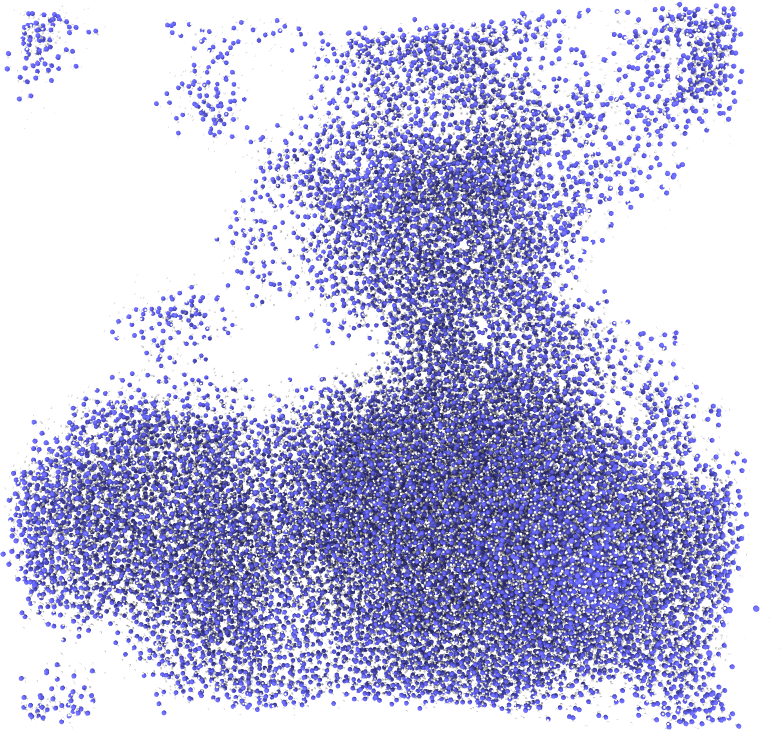
\includegraphics[width=\textwidth]{images/systems/trimmed-rough_fracture01_abel_17}%
%         \caption{Caption.}%
% %         \label{fig:hex_to_tetra}%
%     \end{subfigure}%
%     \caption{%
%         rough\_fracture\_01\_abel - ``Rough fracture \#1'' \hl{Caption} %
%         \label{fig:renderings_rough_fracture01_abel}%
%     }%
% \end{figure}%